
\section{Diagrammi di Sequenza}

Nei diagrammi di sequenza viene mostrata l'interazione fra le classi di design e i componenti del sistema per la realizzazione degli use case del sistema.

In figura~\ref{fig:sequenza:bonifico-sepa} viene illustrata la procedura per l'esecuzione di un bonifico SEPA da parte di un cliente di HBS, parte dell'use case \iducDISPAG.
La query OBP \`e costruita come descritto nella sezione~\ref{sec:OBP}, in particolare dalla figura~\ref{fig:operazioni:bonifico-internazionale:json}.
Il diagramma di sequenza per l'esecuzione di altre tipologie di pagamento differisce dal diagramma in figura~\ref{fig:sequenza:bonifico-sepa} unicamente nella procedura di creazione della query OBP.

\begin{figure*}[h]
    \centering
	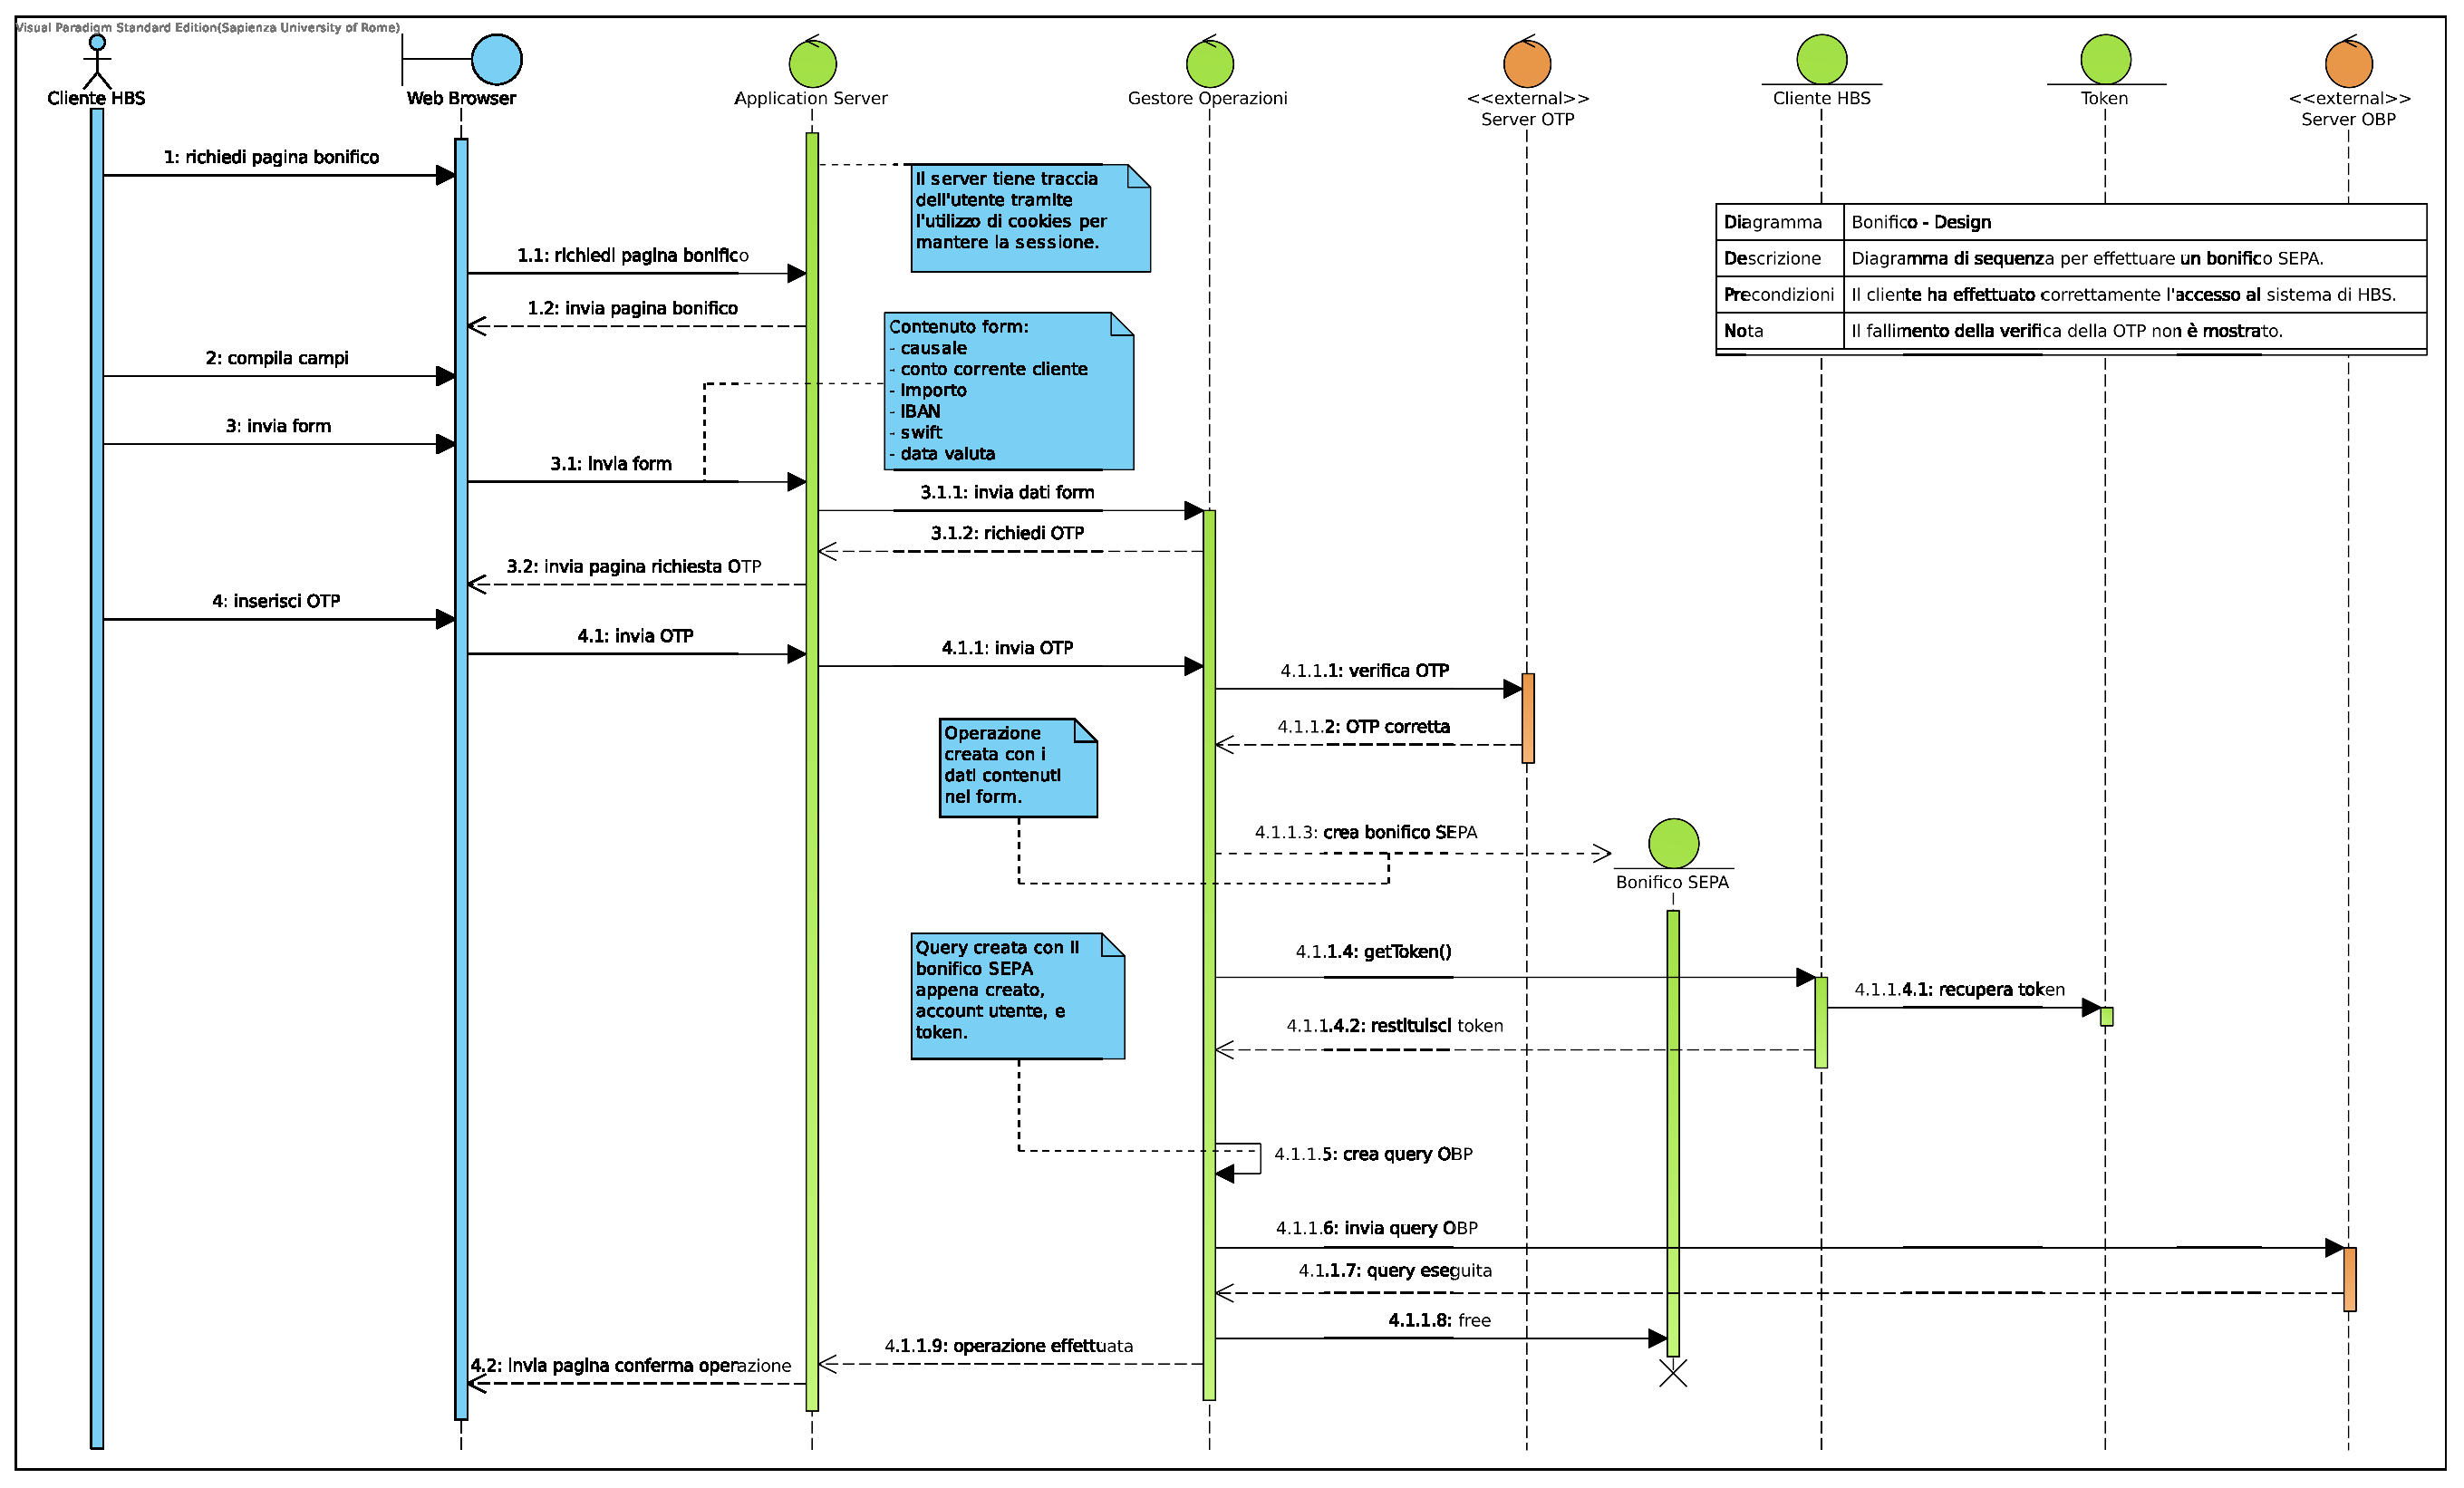
\includegraphics[width=\textheight, angle=90]{Images/Bonifico_-_Design.eps}
    \caption{Diagramma di sequenza relativo all'invio di un bonifico SEPA.}
    \label{fig:sequenza:bonifico-sepa}
\end{figure*}

In figura~\ref{fig:sequenza:saldo} viene illustrata la proceura per ottenere il saldo attuale di un conto corrente, parte dello use case \iducVERSAL.

\begin{figure*}[h]
    \centering
	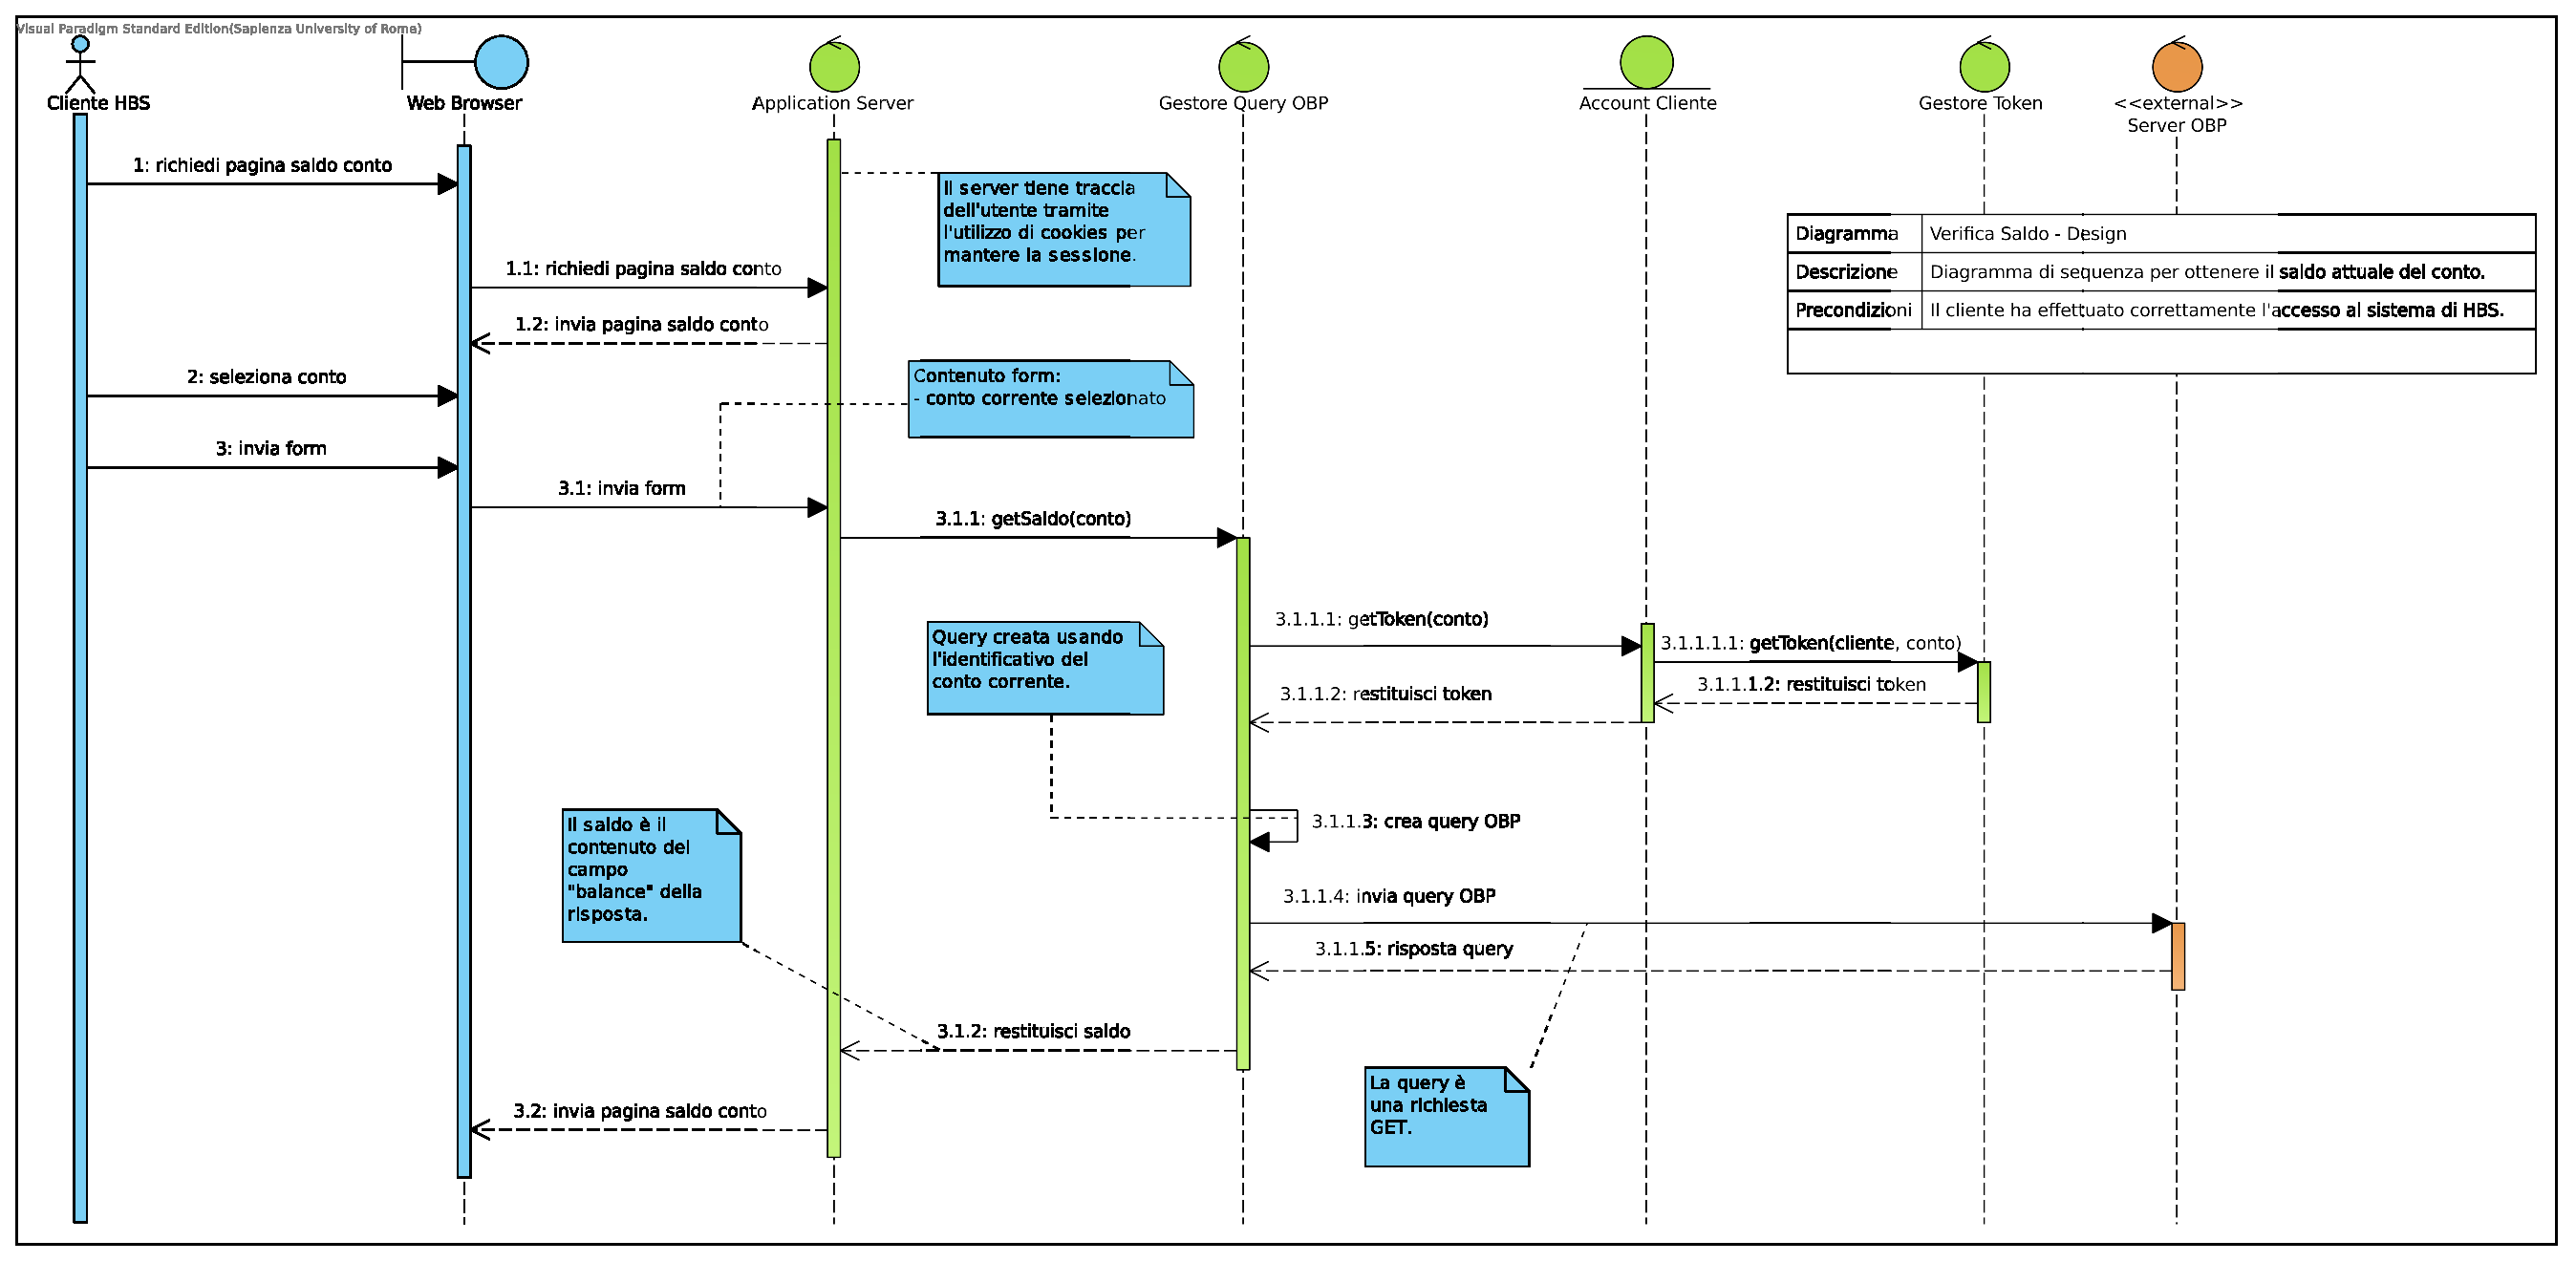
\includegraphics[width=\textheight, angle=90]{Images/Verifica_Saldo_-_Design.eps}
    \caption{Diagramma di sequenza relativo alla verifica del saldo di un conto corrente.}
    \label{fig:sequenza:saldo}
\end{figure*}

In figura~\ref{fig:sequenza:storico} viene illustrata la proceura per ottenere una lista delle transazioni effettuate da un certo conto corrente in un periodo di riferimento, parte dello use case \iducVERSTOR.

\begin{figure*}[h]
    \centering
	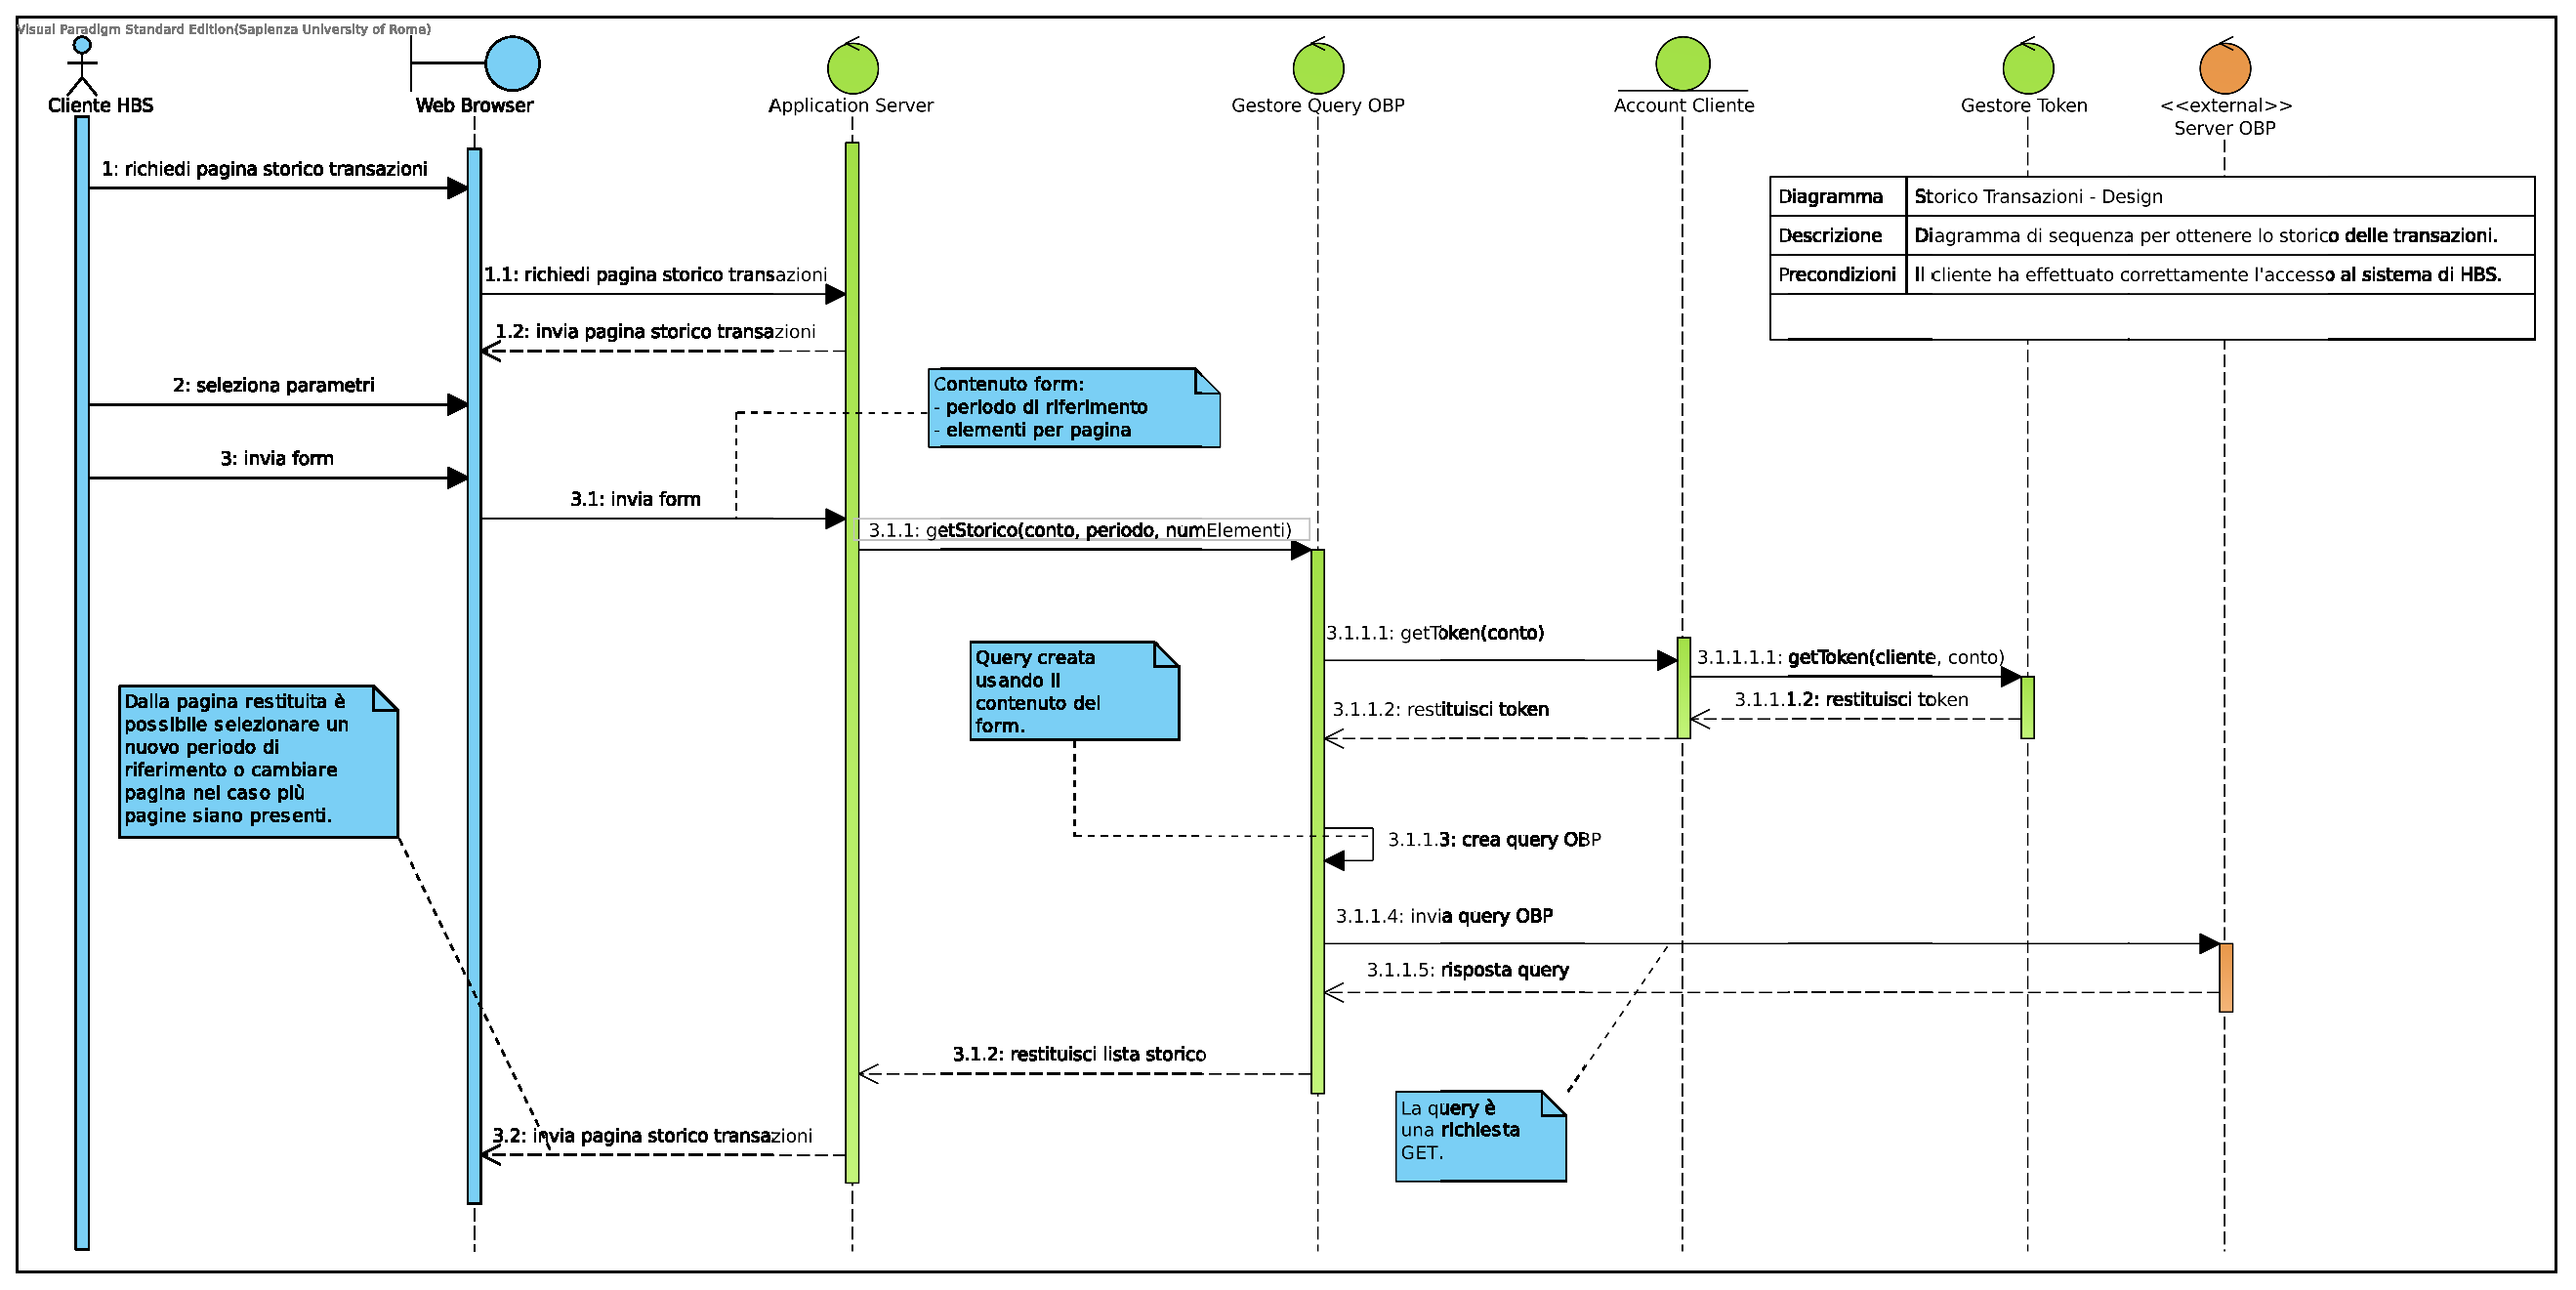
\includegraphics[width=\textheight, angle=90]{Images/Storico_Transazioni_-_Design.eps}
    \caption{Diagramma di sequenza relativo alla visualizzazione dello storico delle transazioni da un conto corrente.}
    \label{fig:sequenza:storico}
\end{figure*}

In figura~\ref{fig:sequenza:log} \`e illustrata la procedura per la creazione di un rapporto destinato al Cliente di HBS partendo dai log mantenuti dal sistema.

\begin{figure*}[h]
    \centering
	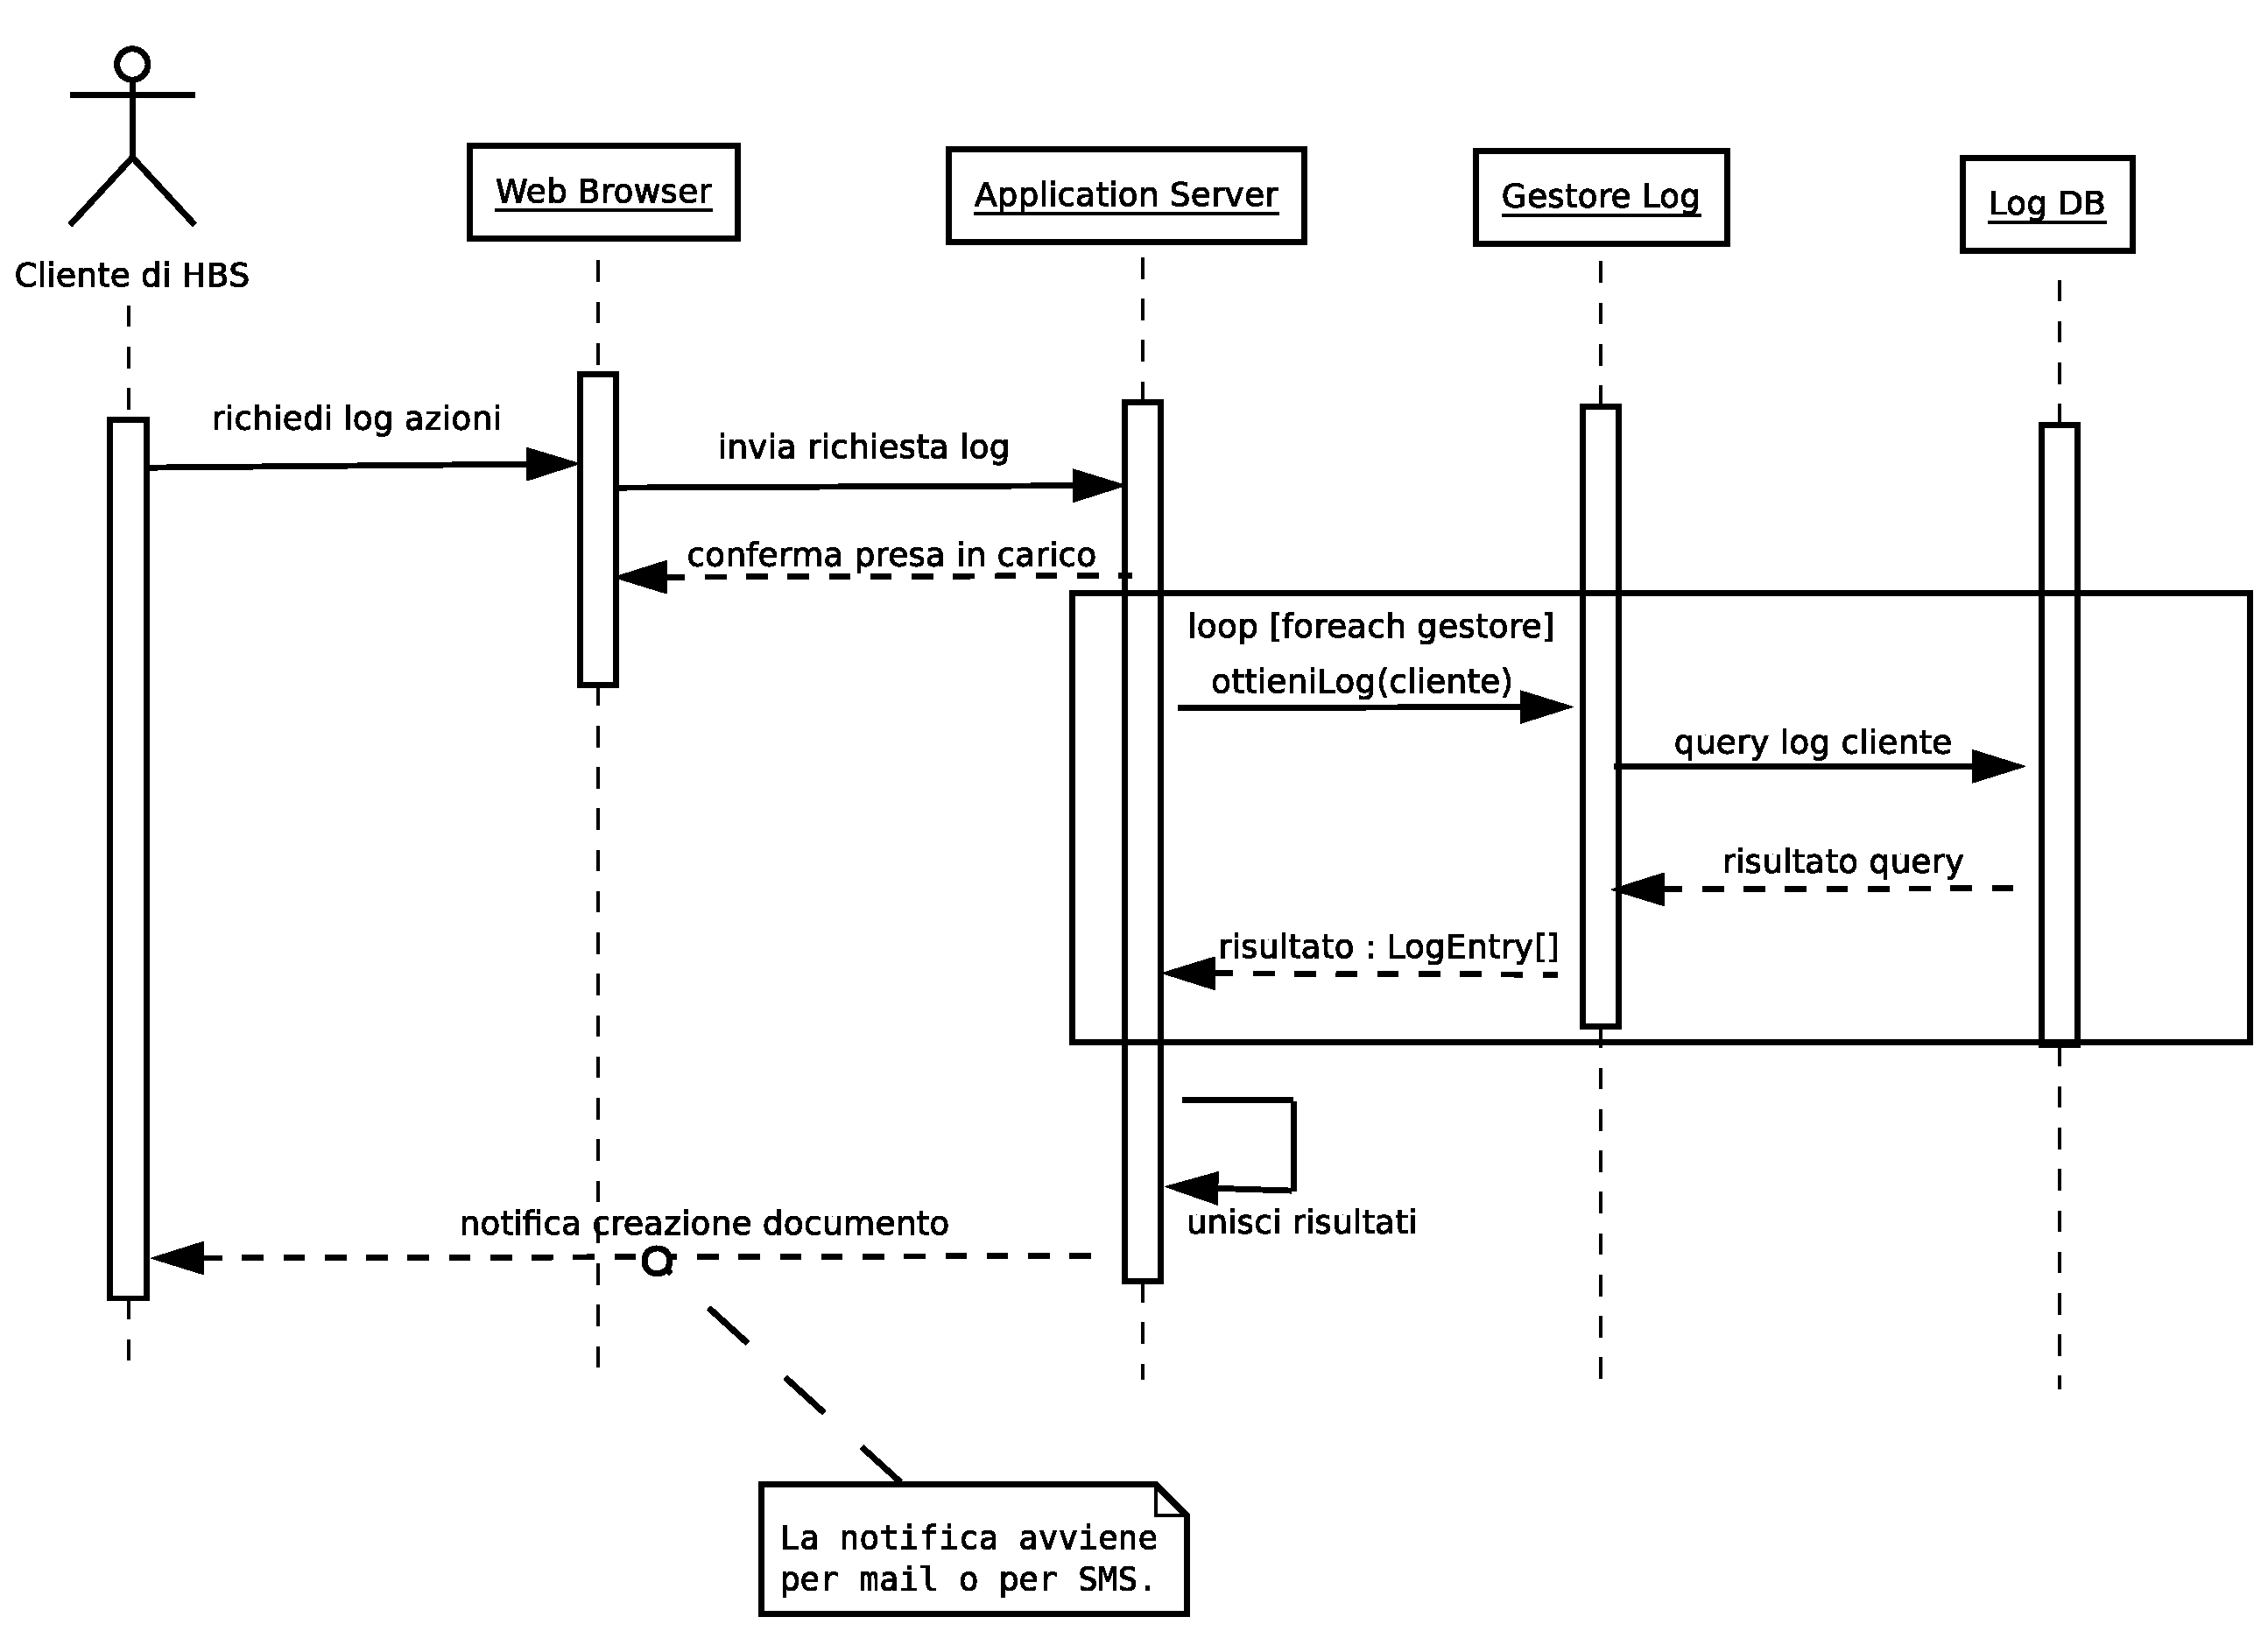
\includegraphics[height=\textwidth, angle=90]{Images/dia/Logging-Sequence.eps}
    \caption{Diagramma di sequenza relativo all'ottenimento del log delle azioni effettuate sul conto dell'utente.}
    \label{fig:sequenza:log}
\end{figure*}


